%%%%%%%%%%%%%%%%%%%%%%%%%%%%%%%%%%%%%%%%%
% Beamer Presentation - S7 Project Phase I
% Project: Ledger - AI-Based Fake News Detection System
% Group: Group 12 (College of Engineering, Cherthala)
%%%%%%%%%%%%%%%%%%%%%%%%%%%%%%%%%%%%%%%%%

\documentclass{beamer}
\mode<presentation> {
\usetheme{Madrid}
\usecolortheme{default}
}

\usepackage{graphicx} % Allows including images
\graphicspath{{diagrams/}{../diagrams/}{./}}
\usepackage{booktabs} % Allows the use of \toprule, \midrule and \bottomrule in tables
\usepackage{textpos}
\usepackage{hyperref}

% PDF Metadata
\hypersetup{
    pdftitle={Ledger - AI-Based Fake News Detection System},
    pdfauthor={Anandhakrishnan S, Aravind A Kamath, Arjun Manoj, Sangeeth Krishnan S},
    pdfsubject={Project Phase I - Zeroth Presentation with Literature Survey},
    pdfkeywords={Fake News Detection, Deep Learning, FastText, CNN, LSTM, Explainable AI, LIME, Literature Survey, CEC}
}

%-------------------------------------------------------------------------------
%	TITLE PAGE
%-------------------------------------------------------------------------------
\begin{document}

\title[BTech S7 Project Phase I]
{\vspace{0.15cm}Ledger - AI-Based Fake News Detection System}

\author[Group 12] { 
  Group 12
  \newline \newline\scriptsize{ Anandhakrishnan S : CEC23CS033
  \newline Aravind A Kamath : CEC23CS041
  \newline Arjun Manoj : CEC23CS043
  \newline Sangeeth Krishnan S : CEC23CS105} \newline
  {\\\footnotesize{Under the Guidance of\\Mrs. Rajeswary R, Assistant Professor}} 
}

\institute[]{

\includegraphics[scale=0.20]{CEC_Logo.jpeg}\\\footnotesize{Dept. of Computer Science and Engineering\\College of Engineering, Cherthala}
}

\date{}

% Slide 1: Title
\begin{frame}
\titlepage 
\end{frame}

% Slide 2: Overview (Table of Contents)
\begin{frame}
\frametitle{Overview}
\tableofcontents
\end{frame}

%-------------------------------------------------------------------------------
%	1. INTRODUCTION
%-------------------------------------------------------------------------------
\section{Introduction}
\begin{frame}
\frametitle{Introduction}
\large{
\begin{itemize}
    \item Digital platforms (such as social media, news pages) have become primary sources of news,
enabling rapid and unchecked spread of misinformation.
    \item Traditional fact-checking relies heavily on manual human verification, which is slow, labor-intensive and unable to scale with viral content.
    \item Fake news influences elections, propagates medical myths (anti-vaccine content, false disease cures), leads to violence (such as riots) and other such negative consequences.
    \item Most AI classifiers offer high predictive accuracy but operate as opaque black boxes, limiting public and institutional trust. That is, we do not know 'why' AI made the decision.
    \item \textbf{Ledger} addresses this gap by combining high-accuracy hybrid deep learning with Explainable AI (XAI) to provide real-time, interpretable fake news verification.
\end{itemize}
}
\end{frame}

%-------------------------------------------------------------------------------
%	2. PROBLEM STATEMENT
%-------------------------------------------------------------------------------
\section{Problem Statement}
\begin{frame}
\frametitle{Problem Statement}
\large{
\begin{itemize}
    \item The spread of fabricated (fake) news severely disrupts democratic elections, promotes harmful medical myths and incites communal unrest.
    \item Both the UN and WHO have designated misinformation/infodemics as critical global public health and democratic threats.
    \item Developing nations like India face greater vulnerability due to the massive population which is having uneven digital media literacy/knowledge.
    \item Existing automated detection tools fail to explain why a given news article was classified as fake, preventing user credibility and adoption.
\end{itemize}
}
\end{frame}

%-------------------------------------------------------------------------------
%	3. LITERATURE SURVEY
%-------------------------------------------------------------------------------
\section{Literature Survey}

% Base Paper (Primary Reference)
\begin{frame}
\frametitle{Base Paper}
\large{
\begin{itemize}
    \item \textbf{Title:} Advancing Fake News Detection: Hybrid Deep Learning With FastText and Explainable AI
    \item \textbf{Author:} Ehtesham Hashmi, Sule Yildirim Yayilgan, Muhammad Mudassar Yamin, Subhan Ali, Mohamed Abomhara
    \item \textbf{Published:} IEEE Access (Volume 12, pp. 44463--44481)
    \item \textbf{Year:} 2024
\end{itemize}
}
\end{frame}

\begin{frame}
\frametitle{Base Paper: Overview}
\small{
\begin{itemize}
    \item \textbf{Key Concepts:} Hybrid Deep Learning architecture combining FastText word embeddings with CNN and LSTM, benchmarked against Transformers and interpreted via Explainable AI (LIME) and LDA topic modeling.
    \item \textbf{Methodology:} Text preprocessing (regex cleaning, lemmatization, tokenization) $\rightarrow$ Subword FastText embeddings $\rightarrow$ 1D-CNN (n-gram feature extraction) $\rightarrow$ LSTM (contextual dependencies) $\rightarrow$ Dense Softmax classification $\rightarrow$ LIME feature attribution.
    \item \textbf{Advantages:}
    \begin{itemize}
        \item Achieves outstanding performance: 99\% accuracy on WELFake, 97\% on FakeNewsNet and 99\% on FakeNewsPrediction.
        \item FastText subwords effectively overcome Out-Of-Vocabulary (OOV) and structural issues in noisy text.
        \item LIME visual attribution provides transparent word-level reasoning, establishing user credibility.
    \end{itemize}
\end{itemize}
}
\end{frame}

\begin{frame}
\frametitle{Base Paper: Limitations}
\large{
\begin{itemize}
    \item Evaluated mostly in English corpora; lacks multiple language support for regional and other languages.
    \item Classifier is susceptible to over-weighting or over-prioritizing superficial keywords (e.g., date/month references or specific proper nouns) in short texts.
    \item Does not consider multimodal attributes (manipulated images, synthetic video) or social propagation graph dynamics.
\end{itemize}
}
\end{frame}

\begin{frame}
\frametitle{Literature Survey}
\fontsize{30pt}{36pt}\selectfont
\centerline{Literature Survey}
\end{frame}

% Paper 1
\begin{frame}
\frametitle{1. Exploiting Stance Similarity and Graph Neural Networks for Fake News Detection}
\framesubtitle{Kazuki Soga, Suguru Yoshida, Masahiro Muneyasu, 2024, Pattern Recognition Letters (Elsevier)}
\small{
\textbf{Key Concepts:} Uses graph-based models to analyze user opinions and news propagation on social networks. \par\vspace{0.15cm}
\textbf{Methodology:} Creates interaction graphs between news articles and users using comments, network structure and stance similarity. \par\vspace{0.15cm}
\textbf{Advantages:}
\begin{itemize}
    \item Uses crowd reactions in addition to news content.
    \item Achieves better F1-scores than traditional CNN/RNN models.
    \item More resistant to adversarial text manipulation.
\end{itemize}
}
\end{frame}

\begin{frame}
\frametitle{1. continuation of Exploiting Stance Similarity and GNNs for Fake News Detection}
\large{
\textbf{Limitations:}
\begin{itemize}
    \item Requires user interactions and social network data.
    \item Needs high memory and computational resources for large graphs.
    \item Cannot effectively handle newly published articles with no user interaction.
\end{itemize}
}
\end{frame}

% Paper 2
\begin{frame}
\frametitle{2. Impact of Convolutional Neural Network and FastText Embedding on Text Classification}
\framesubtitle{Muhammad Umer, Zainab Imtiaz, Muhammad Ahmad et al., 2023, Multimedia Tools and Applications}
\small{
\textbf{Key Concepts:} Combines FastText word embeddings with 1D-CNNs for noisy and unstructured text data classification. \par\vspace{0.15cm}
\textbf{Methodology:} Uses pre-trained FastText embeddings with multi-kernel CNN layers, max-pooling and dropout. \par\vspace{0.15cm}
\textbf{Advantages:}
\begin{itemize}
    \item Handles unknown words, spelling errors and typos (typing mistakes) effectively.
    \item Faster training and inference compared to large transformer models.
    \item Achieves over 94.5% accuracy on text classification benchmarks.
\end{itemize}
}
\end{frame}

\begin{frame}
\frametitle{2. continuation of Impact of CNN and FastText Embedding on Text Classification}
\large{
\textbf{Limitations:}
\begin{itemize}
    \item Captures mainly local text patterns and misses long-range context.
    \item Performance is sensitive to hyperparameter settings.
    \item Cannot effectively understand ambiguous words (words that have multiple/many meanings) in complex sentences.
\end{itemize}
}
\end{frame}

% Paper 3
\begin{frame}
\frametitle{3. A Systematic Survey on Explainable AI Applied to Fake News Detection}
\framesubtitle{S. D. Madhu Kumar, Angel Mary Chacko, 2023, Engineering Applications of AI (Elsevier)}
\small{
\textbf{Key Concepts:} Reviews XAI techniques such as LIME, SHAP and attention maps for fake news detection. \par\vspace{0.15cm}
\textbf{Methodology:} Evaluates different explanation methods, feature attribution techniques and user trust across deep learning models. \par\vspace{0.15cm}
\textbf{Advantages:}
\begin{itemize}
    \item Helps identify misleading linguistic patterns and model biases.
    \item Defines criteria for evaluating explanation quality and reliability.
    \item Improves transparency and user trust in automated fact-checking.
\end{itemize}
}
\end{frame}

\begin{frame}
\frametitle{3. continuation of A Systematic Survey on Explainable AI Applied to Fake News Detection}
\large{
\textbf{Limitations:}
\begin{itemize}
    \item Methods like LIME can slow down real-time predictions.
    \item Explanation quality may vary depending on settings and sample sizes.
    \item No standard method exists to measure human trust in explanations.
\end{itemize}
}
\end{frame}

% Paper 4
\begin{frame}
\frametitle{4. Big Data ML-Based Fake News Detection Using Distributed Learning}
\framesubtitle{Abdullah Altheneyan, Abdullah Alhadlaq, 2023, IEEE Access}
\small{
\textbf{Key Concepts:} Uses Apache Spark and multiple machine learning models for large-scale news classification. \par\vspace{0.15cm}
\textbf{Methodology:} Combines Random Forest, Naive Bayes and Gradient Boosted Trees using TF-IDF and N-gram features. \par\vspace{0.15cm}
\textbf{Advantages:}
\begin{itemize}
    \item Can efficiently process large volumes of social media and news data.
    \item Ensemble approach improves accuracy and reduces model errors.
    \item Achieved 92.4\% accuracy on the FNC-1 dataset.
    \item Suitable for large-scale enterprise applications.
\end{itemize}
}
\end{frame}

\begin{frame}
\frametitle{4. continuation of Big Data ML-Based Fake News Detection Using Distributed Learning}
\large{
\textbf{Limitations:}
\begin{itemize}
    \item Traditional text features may miss deeper contextual meaning.
    \item Requires complex distributed infrastructure and maintenance.
    \item Does not provide clear explanations for individual predictions.
\end{itemize}
}
\end{frame}

% Paper 5
\begin{frame}
\frametitle{5. WELFake: Word Embedding Over Linguistic Features for Fake News Detection}
\framesubtitle{Pawan Kumar Verma, Prateek Agrawal, Ivone Amorim, Radu Prodan, 2021, IEEE TCSS}
\small{
\textbf{Key Concepts:} Hybrid text authentication merging linguistic/statistical characteristics with dense word embeddings to classify fake/deceptive news. \par\vspace{0.15cm}
\textbf{Methodology:} Aggregated 72,134 news records across 4 benchmark sources (Kaggle, McIntire, Reuters, BuzzFeed). Feature concatenation of GloVe/Word2Vec embeddings with 20+ linguistic attributes fed into ensemble and deep learning classifiers. \par\vspace{0.15cm}
\textbf{Advantages:}
\begin{itemize}
    \item Created WELFake, one of the largest balanced open-access benchmark datasets, helping reduce classifier overfitting.
    \item Achieved a high accuracy of 96.73\%, outperforming base/standalone BERT and CNN models by up to 4.25\%.
    \item Showed strong ability to generalize across different types of datasets and domains.
\end{itemize}
}
\end{frame}

\begin{frame}
\frametitle{5. continuation of WELFake: Word Embedding Over Linguistic Features for Fake News Detection}
\large{
\textbf{Limitations:}
\begin{itemize}
    \item Manually extracting linguistic features requires significant time and computational resources.
    \item Does not provide clear explanations for individual predictions, limiting model interpretability (doesn't say why it made that decision).
    \item Fixed word embeddings struggle to understand new words, unknown terms and evolving internet slang.
\end{itemize}
}
\end{frame}

% Paper 6
\begin{frame}
\frametitle{6. FakeBERT: Fake News Detection in Social Media using BERT and Deep Learning}
\framesubtitle{Rohit Kumar Kaliyar, Anurag Goswami, Pratik Narang, 2021, Soft Computing (Springer)}
\small{
\textbf{Key Concepts:} Combines BERT's contextual understanding with CNN-based feature extraction. \par\vspace{0.15cm}
\textbf{Methodology:} Fine-tunes BERT and passes its embeddings through parallel CNN layers with different filter sizes. \par\vspace{0.15cm}
\textbf{Advantages:}
\begin{itemize}
    \item Captures both long-range context and local semantic patterns.
    \item Achieved up to 98.90\% accuracy on benchmark datasets.
    \item Performs well against deceptive writing styles and text manipulation.
\end{itemize}
}
\end{frame}

\begin{frame}
\frametitle{6. continuation of FakeBERT: Fake News Detection in Social Media using BERT and Deep Learning}
\large{
\textbf{Limitations:}
\begin{itemize}
    \item Requires high computational power and GPU memory.
    \item Acts as a black box with limited prediction transparency (reason for AI's decision is not fully shown).
    \item Slower inference makes real-time deployment more difficult.
\end{itemize}
}
\end{frame}

% Paper 7
\begin{frame}
\frametitle{7. Fake News Detection: A Hybrid CNN-RNN Based Approach}
\framesubtitle{Jamal Abdul Nasir, Osama Subhani Khan, Iraklis Varlamis, 2021, Elsevier (IJIM Data Insights)}
\small{
\textbf{Key Concepts:} Combines CNN and RNN/LSTM models to capture both local phrase patterns and long-term sentence context. \par\vspace{0.15cm}
\textbf{Methodology:} Passes word embeddings through CNN layers to extract key phrases, followed by LSTM layers to understand sequential meaning across the whole article. \par\vspace{0.15cm}
\textbf{Advantages:}
\begin{itemize}
    \item Successfully learns both local word combinations and the overall flow of sentences.
    \item Outperforms standalone CNN and RNN models on real-world datasets (such as ISOT).
    \item Achieves high detection accuracy without needing external social media data.
\end{itemize}
}
\end{frame}

\begin{frame}
\frametitle{7. continuation of Fake News Detection: A Hybrid CNN-RNN Based Approach}
\large{
\textbf{Limitations:}
\begin{itemize}
    \item Functions as a black-box model without built-in explanation tools.
    \item Uses standard word embeddings that struggle with spelling mistakes and new internet words.
    \item Requires higher training time on very long news articles.
\end{itemize}
}
\end{frame}

% Paper 8
\begin{frame}
\frametitle{8. FakeNewsNet: A Data Repository with Diverse Features in Social Media for Fake News Detection}
\framesubtitle{Kai Shu, Deepak Mahudeswaran, Suhang Wang, Dongwon Lee, Huan Liu, 2020, Big Data (Mary Ann Liebert)}
\small{
\textbf{Key Concepts:} Combines news content, social networks and information spreading patterns. \par\vspace{0.15cm}
\textbf{Methodology:} Uses linguistic features, publisher credibility, user interactions and news propagation patterns from PolitiFact and GossipCop. \par\vspace{0.15cm}
\textbf{Advantages:}
\begin{itemize}
    \item Provides 23,196 verified news instances with fact-checking information.
    \item Supports analysis of both news content and social media propagation.
    \item Provides a standard benchmark for social context-aware fake news research.
\end{itemize}
}
\end{frame}

\begin{frame}
\frametitle{8. continuation of FakeNewsNet: A Data Repository for Fake News Detection}
\large{
\textbf{Limitations:}
\begin{itemize}
    \item Missing social media data due to API limits and deleted posts.
    \item Depends heavily on external social media data, making text-only verification difficult.
    \item Some domain subsets have imbalanced classes.
\end{itemize}
}
\end{frame}

% Paper 9
\begin{frame}
\frametitle{9. Supervised Learning for Fake News Detection: An Explainable Approach}
\framesubtitle{Julio C. S. Reis, André Correia, Fabrício Murai et al., 2019, IEEE Internet Computing}
\small{
\textbf{Key Concepts:} Analyzes which text features (such as writing style, grammar and emotion) are most useful for detecting fake news. \par\vspace{0.15cm}
\textbf{Methodology:} Extracts linguistic, syntactic and sentiment features from news articles and evaluates their importance using machine learning models. \par\vspace{0.15cm}
\textbf{Advantages:}
\begin{itemize}
    \item Helps identify which writing characteristics most strongly indicate deceptive news.
    \item Provides understandable feature importance rankings instead of purely opaque predictions.
    \item Shows that sensational and emotional language is a strong signal of fake news.
\end{itemize}
}
\end{frame}

\begin{frame}
\frametitle{9. continuation of Supervised Learning for Fake News Detection: An Explainable Approach}
\large{
\textbf{Limitations:}
\begin{itemize}
    \item Relies heavily on manual feature engineering rather than automated deep learning.
    \item Achieves lower accuracy on complex sentences compared to modern deep neural networks.
    \item Explains overall feature importance rather than highlighting specific suspicious words in real time.
\end{itemize}
}
\end{frame}

% Paper 10
\begin{frame}
\frametitle{10. "Liar, Liar Pants on Fire": A New Benchmark Dataset for Fake News Detection}
\framesubtitle{William Yang Wang, 2017, ACL (Association for Computational Linguistics)}
\small{
\textbf{Key Concepts:} Introduces the LIAR benchmark dataset for fake news detection with multiple truthfulness levels. \par\vspace{0.15cm}
\textbf{Methodology:} Collected 12,800 short statements from PolitiFact, classified into 6 truth levels using standard machine learning and deep learning models (such as CNNs). \par\vspace{0.15cm}
\textbf{Advantages:}
\begin{itemize}
    \item Provides a large, high-quality benchmark dataset with detailed fact-checker ratings.
    \item Tests both surface-level text features and speaker information.
    \item Widely used as a standard dataset to evaluate fake news detection algorithms.
\end{itemize}
}
\end{frame}

\begin{frame}
\frametitle{10. continuation of "Liar, Liar Pants on Fire" Dataset Study}
\large{
\textbf{Limitations:}
\begin{itemize}
    \item Short statements often lack enough context for deep language understanding.
    \item Text-only models struggle to achieve high accuracy without extra metadata (such as speaker history).
    \item Does not provide automated visual explanations for why a statement is fake.
\end{itemize}
}
\end{frame}

%-------------------------------------------------------------------------------
%	4. EXISTING SYSTEM
%-------------------------------------------------------------------------------
\section{Existing System}
\begin{frame}
\frametitle{Existing System}
\large{
\begin{itemize}
    \item \textbf{Manual Fact-Checking:} Platforms rely on human reviewers, which is slow and cannot keep up with viral fake news.
    \item \textbf{Black-Box AI Models:} Current deep learning and Transformer models give predictions without explaining why an article is real or fake.
    \item \textbf{High Resource Requirements:} Heavy transformer models require expensive GPUs and are too slow for real-time consumer web applications.
    \item \textbf{Dependence on Social Media Data:} Many systems require user comments, shares or network graphs, making them unusable for newly published standalone news.
    \item \textbf{Vulnerability to Typos and Slang:} Traditional word embeddings fail to handle misspelled words, new slang and informal social media text.
\end{itemize}
}
\end{frame}

%-------------------------------------------------------------------------------
%	5. PROPOSED SYSTEM
%-------------------------------------------------------------------------------
\section{Proposed System}
\begin{frame}
\frametitle{Proposed System}
\large{
\begin{itemize}
    \item \textbf{Ledger Platform:} A web-based application where users can paste news text or headlines and get instant verification.
    \item \textbf{FastText Subword Embeddings:} Breaks words into subwords to easily handle unknown words, spelling mistakes and internet slang.
    \item \textbf{Hybrid CNN-LSTM Architecture:} Uses CNN layers to capture key phrases and LSTM layers to learn the sequential context of the article.
    \item \textbf{Explainable AI (LIME):} Highlights the exact words and phrases that caused the prediction, making the decision clear and trustworthy.
    \item \textbf{Lightweight and Fast:} Combines a FastAPI backend with a React.js frontend for fast, low-cost and real-time predictions.
\end{itemize}
}
\end{frame}

%-------------------------------------------------------------------------------
%	6. ARCHITECTURE
%-------------------------------------------------------------------------------
\section{Architecture}
\begin{frame}
\frametitle{System Architecture}
\begin{center}
    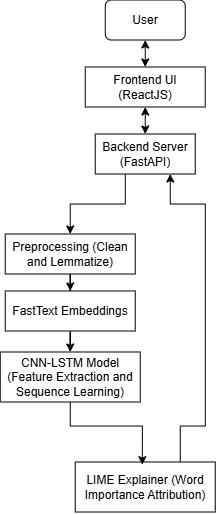
\includegraphics[height=0.76\textheight,keepaspectratio]{ArchitectureDiagram.drawio.png}
\end{center}
\end{frame}

%-------------------------------------------------------------------------------
%	7. METHODOLOGY
%-------------------------------------------------------------------------------
\section{Methodology}
\begin{frame}
\frametitle{Methodology}
\small{
\begin{enumerate}
    \setlength{\itemsep}{2pt}
    \item \textbf{Input Stage:} User submits news text or headline via the web frontend.
    \item \textbf{Text Preprocessing and Embedding:} Tokenization and extraction of FastText subword semantic embeddings.
    \item \textbf{Feature Extraction (CNN):} Convolutional layers capture localized n-gram textual features.
    \item \textbf{Sequence Learning (LSTM):} LSTM layers retain contextual sequence dependencies across the text.
    \item \textbf{Classification:} Dense Softmax layer outputs the predicted label (Real or Fake) with confidence score.
    \item \textbf{Explainability (XAI):} LIME computes word-level feature importance weights.
    \item \textbf{Output Stage:} Frontend displays the authenticity verdict alongside highlighted keywords.
\end{enumerate}
}
\end{frame}

%-------------------------------------------------------------------------------
%	8. DESIGN DIAGRAMS
%-------------------------------------------------------------------------------
\section{Design Diagrams}
\begin{frame}
\frametitle{Data Flow Diagram: Level 0}
\vfill
\begin{center}
    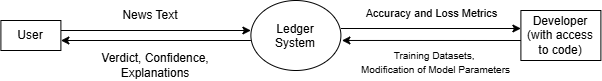
\includegraphics[width=0.95\textwidth,keepaspectratio]{DFD_0.drawio.png}
\end{center}
\vfill
\end{frame}

\begin{frame}
\frametitle{Data Flow Diagram: Level 1}
\vfill
\begin{center}
    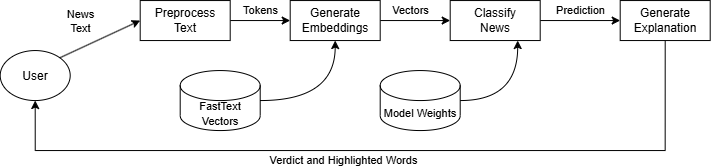
\includegraphics[width=0.95\textwidth,keepaspectratio]{DFD_1.drawio.png}
\end{center}
\vfill
\end{frame}

\begin{frame}
\frametitle{UML Sequence Diagram}
\begin{center}
    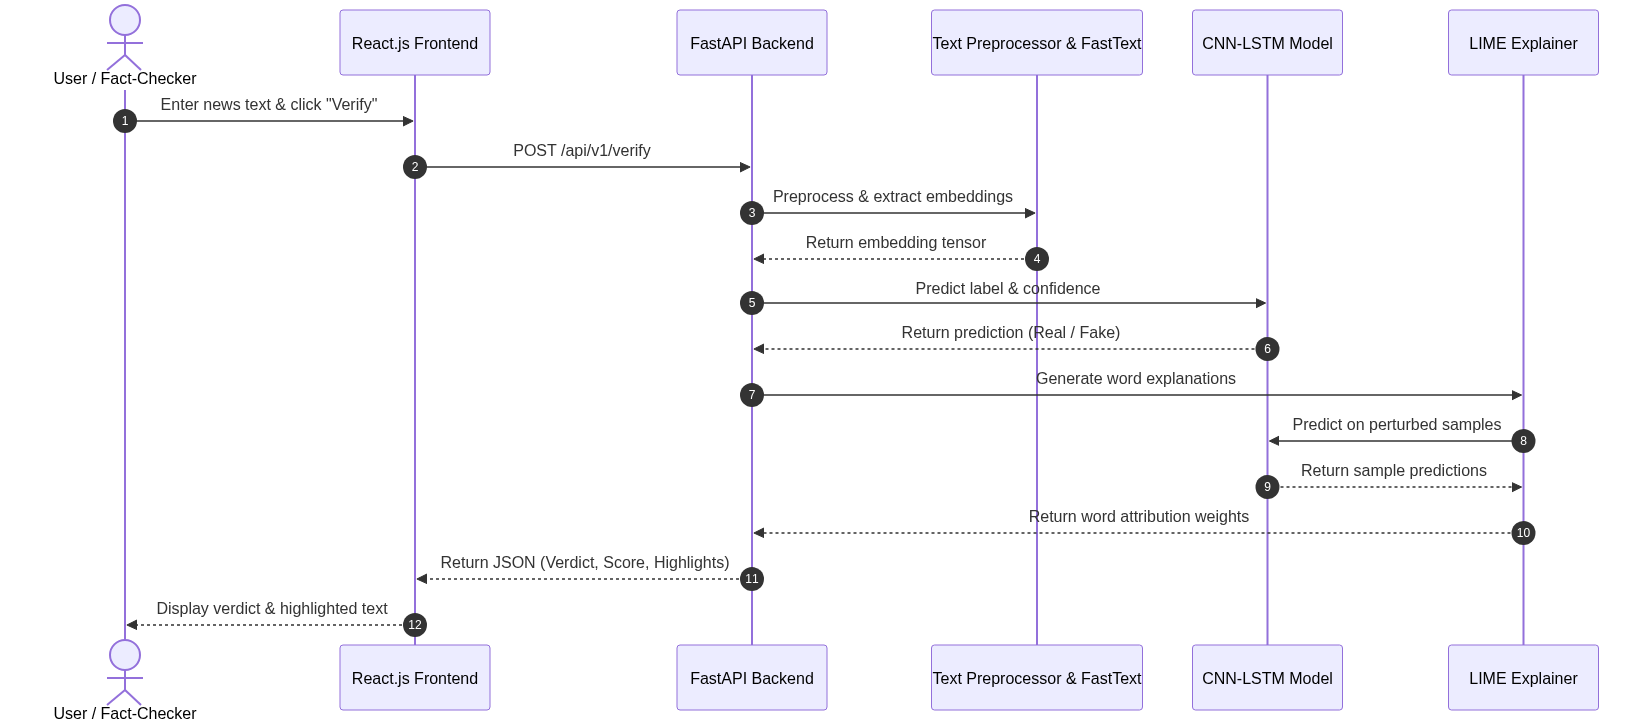
\includegraphics[width=0.95\textwidth,height=0.76\textheight,keepaspectratio]{uml_sequence_diagram.png}
\end{center}
\end{frame}

%-------------------------------------------------------------------------------
%	9. CONCLUSION
%-------------------------------------------------------------------------------
\section{Conclusion}
\begin{frame}
\frametitle{Conclusion}
\large{
\begin{itemize}
    \item The literature highlights a trade-off: high-accuracy transformers and deep networks lack transparency, while interpretable models often underperform.
    \item \textbf{Ledger} resolves this dilemma by integrating \textbf{FastText + CNN-LSTM} for lightweight, state-of-the-art accuracy with \textbf{LIME} for explainability.
    \item Subword embeddings effectively resolve vocabulary gaps (OOV tokens) common in sensationalized social media misinformation.
    \item The proposed end-to-end web system provides everyday users and fact-checkers with instant, interpretable and credible fake news verification.
\end{itemize}
}
\end{frame}

%-------------------------------------------------------------------------------
%	10. REFERENCES
%-------------------------------------------------------------------------------
\section{References}
\begin{frame}[allowframebreaks]
\frametitle{References}
\scriptsize{
\begin{itemize}
    \item \textbf{[Base Paper]} E. Hashmi, S. Y. Yayilgan, M. M. Yamin, S. Ali and M. Abomhara, ``Advancing Fake News Detection: Hybrid Deep Learning With FastText and Explainable AI,'' \textit{IEEE Access}, vol. 12, pp. 44463--44481, 2024.
    \item P. K. Verma, P. Agrawal, I. Amorim and R. Prodan, ``WELFake: Word Embedding Over Linguistic Features for Fake News Detection,'' \textit{IEEE Transactions on Computational Social Systems}, vol. 8, no. 4, pp. 881--893, Aug. 2021.
    \item K. Shu, D. Mahudeswaran, S. Wang, D. Lee and H. Liu, ``FakeNewsNet: A Data Repository with News Content, Social Context and Spatiotemporal Information for Studying Fake News on Social Media,'' \textit{Big Data}, vol. 8, no. 3, pp. 171--188, Jun. 2020.
    \item M. Umer, Z. Imtiaz, M. Ahmad, M. Nappi, C. Medaglia, G. S. Choi and A. Mehmood, ``Impact of Convolutional Neural Network and FastText Embedding on Text Classification,'' \textit{Multimedia Tools and Applications}, vol. 82, no. 4, pp. 5569--5585, Feb. 2023.
    \item R. K. Kaliyar, A. Goswami and P. Narang, ``FakeBERT: Fake News Detection in Social Media using BERT and Deep Learning,'' \textit{Soft Computing}, vol. 25, no. 18, pp. 11771--11788, Sep. 2021.
    \item S. D. M. Kumar and A. M. Chacko, ``A Systematic Survey on Explainable AI Applied to Fake News Detection,'' \textit{Engineering Applications of Artificial Intelligence}, vol. 122, Art. no. 106087, Jun. 2023.
    \item K. Soga, S. Yoshida and M. Muneyasu, ``Exploiting Stance Similarity and Graph Neural Networks for Fake News Detection,'' \textit{Pattern Recognition Letters}, vol. 177, pp. 26--32, Jan. 2024.
    \item A. Altheneyan and A. Alhadlaq, ``Big Data ML-Based Fake News Detection Using Distributed Learning,'' \textit{IEEE Access}, vol. 11, pp. 29447--29463, 2023.
    \item W. Y. Wang, ````Liar, Liar Pants on Fire'': A New Benchmark Dataset for Fake News Detection,'' in \textit{Proc. 55th Annu. Meeting Assoc. Comput. Linguistics (ACL)}, 2017, pp. 422--426.
    \item J. A. Nasir, O. S. Khan and I. Varlamis, ``Fake news detection: A hybrid CNN-RNN based approach,'' \textit{Int. J. Inf. Manage. Data Insights}, vol. 1, no. 2, Art. no. 100032, Nov. 2021.
    \item J. C. S. Reis, A. Correia, F. Murai, A. Veloso and F. Benevenuto, ``Supervised Learning for Fake News Detection: An Explainable Approach,'' \textit{IEEE Internet Computing}, vol. 23, no. 2, pp. 46--53, Mar.--Apr. 2019.
\end{itemize}
}
\end{frame}

%-------------------------------------------------------------------------------
%	THANK YOU
%-------------------------------------------------------------------------------
\begin{frame}
\fontsize{45pt}{60pt}\selectfont
\centerline{Thank You}
\end{frame}

\end{document}